\chapter{A quick travel in the history of crowdsourcing}
\label{chap:history-crowdsourcing}
\section{History of crowdsourcing}
\label{sec:history-of-crowdsourcing}
Crowdsourcing in its most general form is not new. We have records of large crowdsourcing experiments leading to high achievements in socio-economics fields and even playing parts in wars. Let us consider one historical example.

One of the eldest and most impactful happened in 1848 and is reported extensively in \citet{tracksinthesea}. Led by Matthew Fontaine Maury (an oceanographer between many other titles), the U.S. Naval Observatory distributed free copies of his book \emph{Wind and Current Charts} which described how to effectively reduce time travel at sea, see \Cref{fig:wind-current} -- \emph{shippers knew that every day saved at sea cut costs and lessened the danger of losing ships, cargoes and crews}. In return, Maury asked sailors to record standardized logs and return them to him at the U.S. Naval Observatory.
This form came with a ten-page instruction pamphlet on how to interpret the charts and how to fill out the logs.
The experiment ran for years, and even at the early beginning shipmasters wanted to increase their profit and participate: \emph{By September, the logs began flowing into the observatory, and Maury and his staff were busy trying to handle the volume}.
Collecting this information led to reducing the Rio de Janeiro - New York was then fifty-five days and was reduced to twenty-three in 1853.
They simplified and extended the charts with the full support of Navy captains and merchant companies like Forbes of Boston and Robert C. Wright of Baltimore for their sailors to fill out these forms.
More importantly, they noticed some sailors did not use the charts correctly, and this helped prove the importance of taking into account winds and currents at sea.
The newly collected data also helped create monthly recommendation charts for sailors.
\begin{figure}[ht]
    \centering
    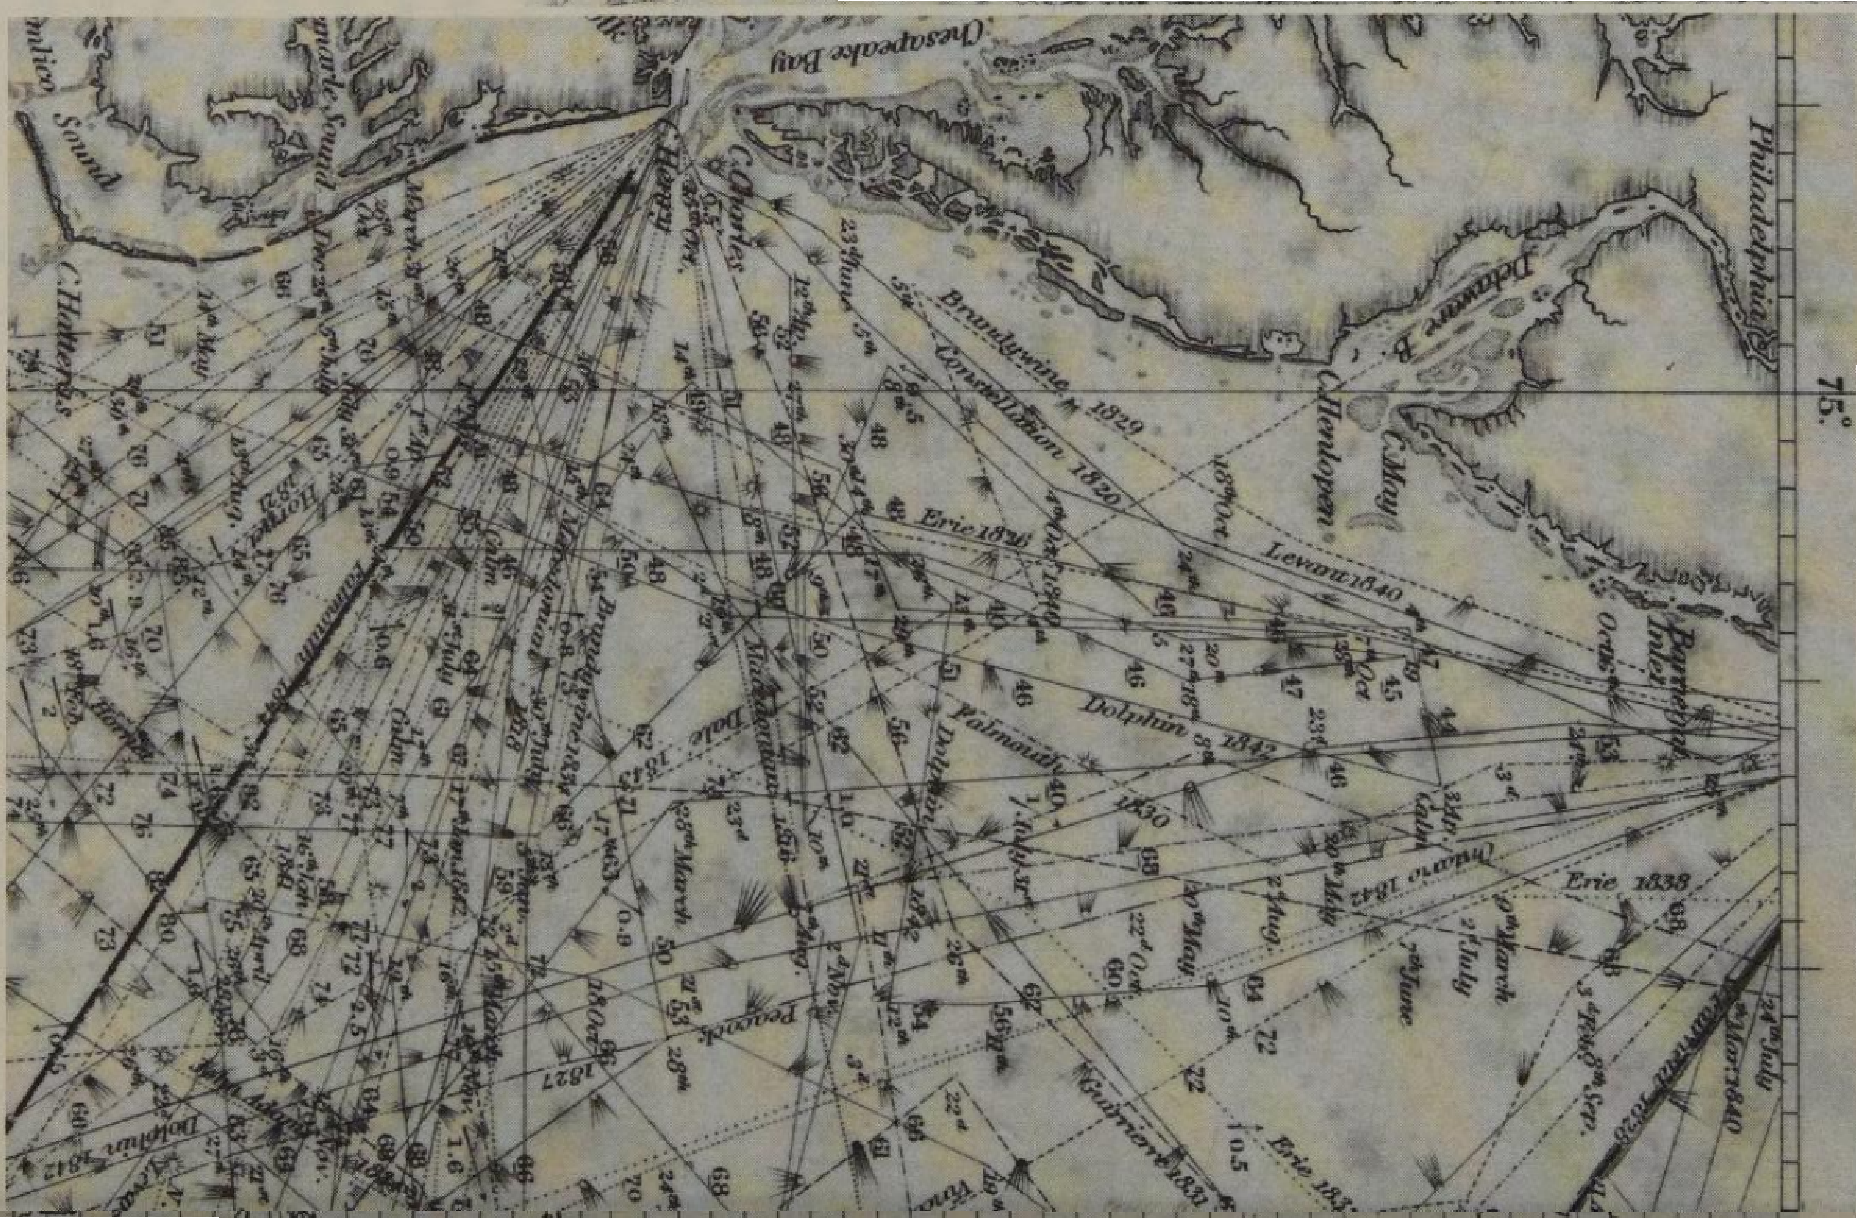
\includegraphics[width=.7\textwidth]{chapters/images/windmaps.pdf}
    \caption{Extract of the first edition of Wind and Current Chart of the North-Atlantic (1848) by Matthew Fontaine Maury. The brushes show the direction wind blows and their strength. The currents are shown with arrows. We can also see the water temperatures around the Chesapeake Bay.}
    \label{fig:wind-current}
\end{figure}

But the history of Maury's logs implications did not stop at currents and winds. In 1851, they released charts showing the distribution of sperm whales in oceans for each season -- an example is shown in \Cref{fig:whale-chart}. These tracks were used by whalers, but also during the Civil War by confederates to track Union ships that captured and harvested animals \footnote{\url{https://www.nytimes.com/1865/08/27/archives/the-pirate-shenandoah-her-cruise-in-the-arctic-seas-wholesale.html}}. This disrupted the North's economy as sperm whale's oil was popular for soaps, lubricants and also as light sources \footnote{\url{https://www.nytimes.com/2008/08/03/nyregion/03towns.html}}.
\begin{figure}[ht]
    \centering
    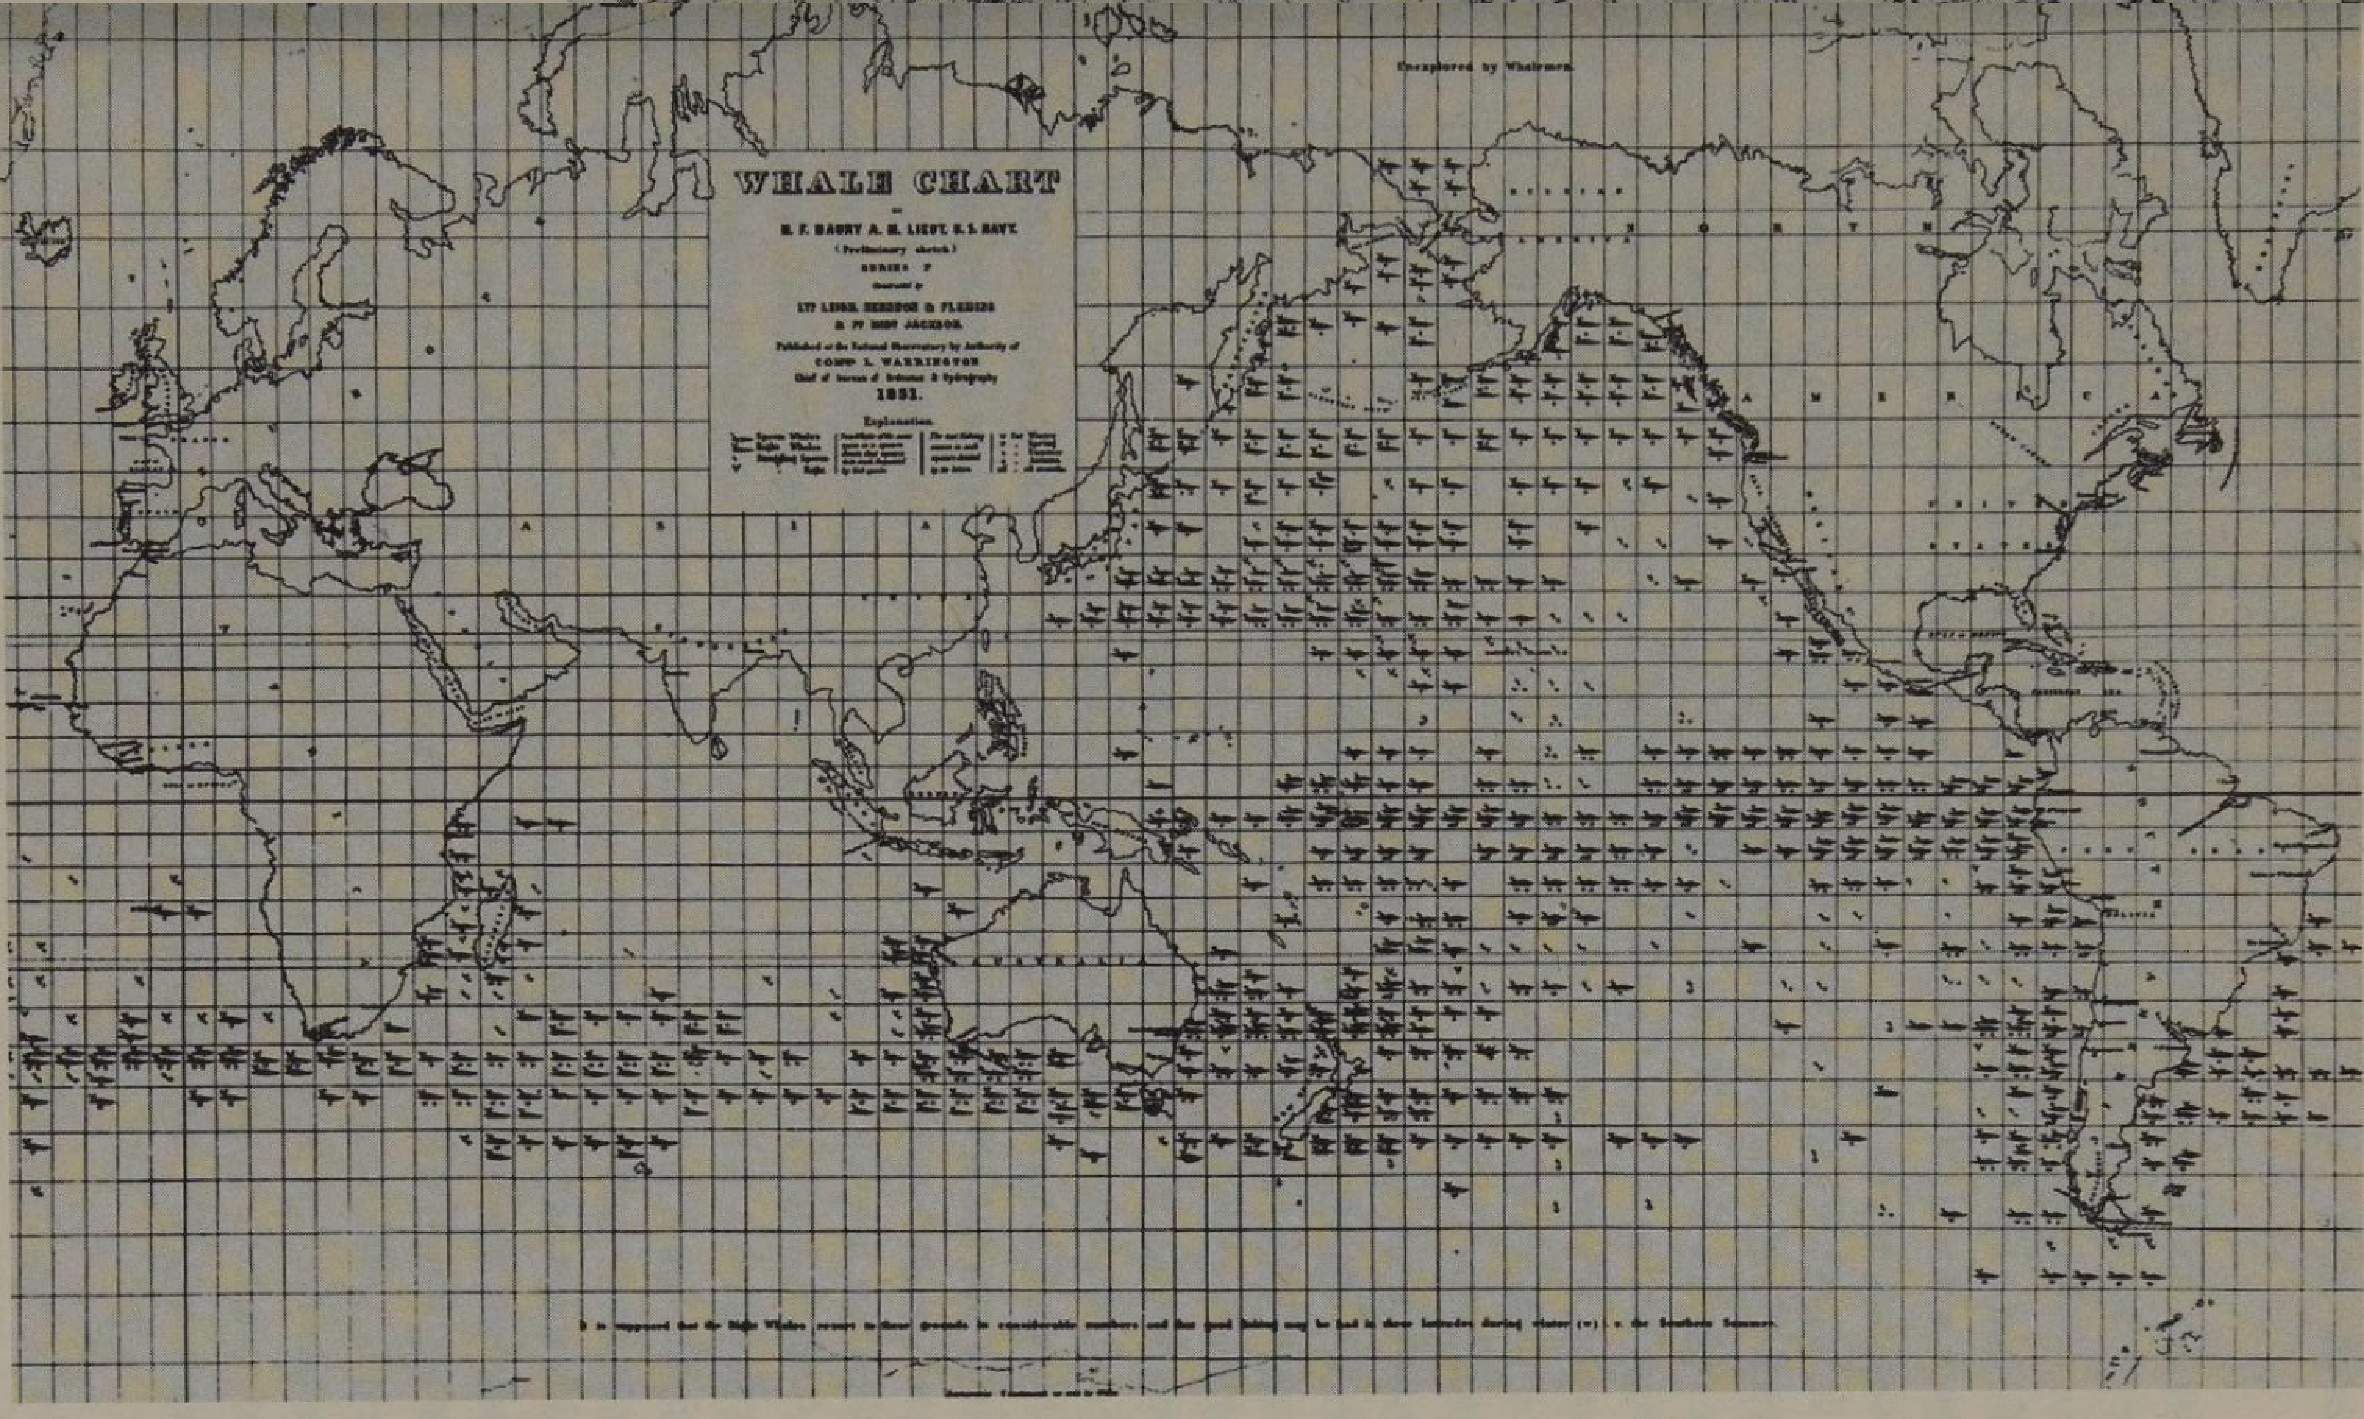
\includegraphics[width=.7\textwidth]{chapters/images/whales.pdf}
    \caption{Whale chart by Matthew Fontaine Maury from 1851, series F showing the distribution of sperm whales across oceans.}
    \label{fig:whale-chart}
\end{figure}

\section{Defining crowdsourcing}
\label{sub:definition-crowdsourcing}

Even though crowdsourcing isn't new, this is not the case for its proposed definition.
Because of its large possibilities of applications and the increasingly extensive use of the internet to conduct crowdsourcing experiments, there are multiple definitions of the term.

One of the first was recorded in 2006 by two journalists at Wired, Jeff Howe and Mark Robinson:
\begin{center}
\begin{minipage}{.75\textwidth}
    \emph{Simply defined, crowdsourcing represents the act of a company or institution taking a function once performed by employees and outsourcing it to an undefined (and generally large) network of people in the form of an open call. This can take the form of peer-production (when the job is performed collaboratively), but is also often undertaken by sole individuals. The crucial prerequisite is the use of the open call format and the large network of potential laborers.}
\end{minipage}
\end{center}
Later, Howe proposed to divide it into two definitions\footnote{\url{https://crowdsourcing.typepad.com/cs/2006/06/crowdsourcing_a.html}}:
\begin{center}
\begin{minipage}{.75\textwidth}
\begin{itemize}
    \item \emph{The White Paper Version: Crowdsourcing is the act of taking a job traditionally performed by a designated agent (usually an employee) and outsourcing it to an undefined, generally large group of people in the form of an open call.
}
    \item \emph{The Soundbyte Version: The application of Open Source principles to fields outside of software.
}
\end{itemize}
\end{minipage}
\end{center}

With the increasing use and misuse of the word crowdsourcing, \citet{estelles2012towards} provided a broader internet-based definition that was extracted from merging definitions from forty papers -- from a database of journal and conference papers about crowdsourcing containing 209 papers. The definition is as follows:
\begin{center}
\begin{minipage}{.75\textwidth}
\emph{
Crowdsourcing is a type of participative online activity in which an individual, an institution, a non-profit
organization, or company proposes to a group of individuals of varying knowledge, heterogeneity, and
number, via a flexible open call, the voluntary undertaking of a task. The undertaking of the task, of variable complexity and modularity, and in which the crowd should participate bringing their work, money, knowledge and/or experience, always entails mutual benefit. The user will receive the satisfaction of a given type of need, be it economic, social recognition, self-esteem, or the development of individual skills, while the crowdsourcer will obtain and utilize to their advantage that what the user has brought to the venture, whose form will depend on the type of activity undertaken.
}
\end{minipage}
\end{center}

One of their criteria was to explicitly take into account the "internet" factor to define modern crowdsourcing, thus this does not apply to experiments like Matthew Fontaine Maury's (\Cref{sec:history-of-crowdsourcing}). However, in the context of this thesis, and given how the vast majority of crowdsourcing experiments are nowadays used thanks to the internet, this definition is sufficient for our research purposes.

More importantly, the definition of crowdsourcing does not include peer production.
These two are often mixed up, but experts \citep{brabham2013crowdsourcing} differentiate them with multiple criteria -- the most important being the guidelines.
Let us take from \citet{brabham2013crowdsourcing} the example of one of the largest peer-production projects: Wikipedia.
It can not be considered a crowdsourcing project as there is no guideline given on what should be in an article or how it should be structured.
There is also no vertical control.
Wikipedia is controlled via peer assessments, so it is a horizontal control through dialogues.
In a crowdsourcing experiment, a crowdsourcer (company, laboratory,\dots) provides the task(s) and what should be done to complete them.
This can be as simple as \emph{Describe the image} or \emph{click on the bike}, or more complicated like \emph{can the second part of the proposition be inferred from the first part?} but the main point is that there is a clear guideline given directly to the worker to complete the task(s) at hand.

\section{Explicit and implicit crowdsourcing}
\label{sub:explicit-and-implicit}

From the multiple definitions of the term crowdsourcing, we see that broad implications lead to multi-faceted types of work.
More than the task itself to be completed, it is important to record how the tasks were presented to workers.
We know from \Cref{sub:definition-crowdsourcing} that a guideline plays a crucial part in the experiment.
However, a guideline can hide the purpose of an experiment. So crowdsourcing has been divided between two categories \citep{andro2017digital}:
\begin{itemize}
    \item implicit crowdsourcing: recourse to involuntary work by Internet users,
    \item explicit crowdsourcing: recourse to voluntary work from voluntary Internet users.
\end{itemize}

A famous example of implicit crowdsourcing tasks is the \texttt{reCAPTCHA} created by Luis von Ahn.
The principle is simple, we need to archive old books, and sometimes text recognition systems can not recognize the words -- for numerous reasons such that, and not exhaustive, paper quality, symbols and calligraphy, overlapping words -- and those words are given to write out to people on the internet just as ordinary security systems (see \Cref{fig:recaptcha}).
Most of the time, there are two \texttt{CAPTCHA}s to solve, one for control and then the actual task.
During the whole solving time, the worker does not know that they are solving an actual problem for a crowdsourcer, hence the implicit.
Multiple other examples for each are presented in \Cref{sub:run-experiments} with a more detailed classification of crowdsourcing tasks.

\begin{figure}[ht]
    \centering
    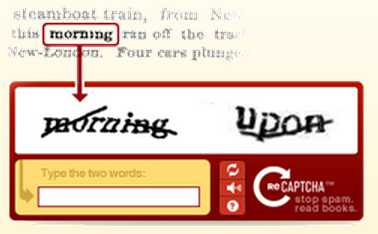
\includegraphics[width=.5\textwidth]{chapters/images/recaptcha.jpg}
    \caption{Example of \texttt{reCAPTCHA} from 2014 for word recognition tasks. The word here is \texttt{morning} and the control word \texttt{upon}.}
    \label{fig:recaptcha}
\end{figure}


\section{Current ways to classify and run experiments}
\label{sub:run-experiments}

Defining types of crowdsourcing is not the same as defining types of crowds.
In \citet{kazai2011worker} created five worker profiles: spammer, sloppy, incompetent, competent, and diligent. In \citet{martineau2012typology} workers are classified as communal, lurkers, utilizers and aspirers.
This quest for worker profile identification is still an active field of research.

But taking a step back in this problem, \citet{brabham2013crowdsourcing} proposes a typology to classify crowdsourcing experiments: not tasks nor workers.
\begin{itemize}
    \item knowledge discovery and management: find and collect standardized information -- \emph{e.g} Flag association application to register discrimination and act of violence against LGBTQ+ people for the French government\footnote{\url{https://www.flagasso.com/}},
    \item broadcast search: solve empirical problems -- \emph{e.g} coding challenges as Kaggle
    \item peer-vetted creative production: create and select creatives ideas -- \emph{e.g} Threadless\footnote{\url{https://www.threadless.com/}} allow its community to create designs for shirts or prints and then puts them to a vote each week,
    \item Distributed-human-intelligence tasking; analyze large amounts of information -- \emph{e.g} label images or part of images like Pl@ntNet.
\end{itemize}

In practice, running a crowdsourcing experiment has been eased up by platforms such as Amazon Mechanical Turk\footnote{\url{https://mkturk.com/}} or Toloka\footnote{\url{https://toloka.yandex.com}}.
These marketplaces allow to conduct of a paid experiment -- ethical considerations apart (and discussed in \cref{sub:ethics}) -- that is planned with extensive parametrization.
The data labeling is outsourced so you don't need to think about the resource allocations. They also have algorithms (some like \citet{raykar_ranking_2011} that we discuss in \Cref{chap:peerannot}) to detect unreliable workers to have better data.

\begin{figure}[ht]
        \centering
        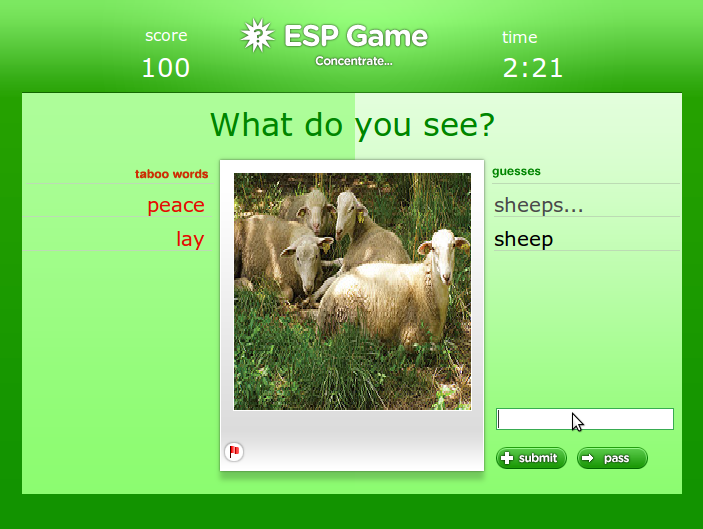
\includegraphics[width=.6\textwidth]{chapters/images/ESP.png}
        \caption{Example of ESP game image (from \url{https://edutechwiki.unige.ch}). The image represents four sheep laying in the grass. The first worker proposes \texttt{sheep} and then \texttt{sheep} at the second round. Note that to avoid having the same labels by multiple workers for the images, taboo words were introduced. In this case, workers were forbidden to answer the words \texttt{peace} and \texttt{lay} to describe the image. Not every image had taboo words.}
        \label{fig:ESP-game}
\end{figure}

However, paying workers is not the only way to collect crowdsourced data.
The gamification of crowdsourcing tasks has proved to be quite efficient with experiments like Eyewire \citep{tinati2017investigation}, ThePlantGame \citep{plantgame2016}, \emph{etc}.
Luis Von Ahn (the \texttt{CAPTCHA} creator) was one of the first researchers on GWAPs (Games With A Purpose).
He famously also founded in 2004 the ESP (ExtraSensory Perception) game \citep{von2005esp} to create metadata on images --  presented in \Cref{fig:ESP-game}.
Two players are paired up randomly and shown the same image.
They can not communicate, but they each can provide a single word to describe the image presented.
Once they both provide the same word, the game stops.
They have 2 minutes and 30 seconds to label 15 images.
At one point, they can both choose to pass on a single image.
A license was bought by Google to create the Google Image Labeler\footnote{\url{http://news.bbc.co.uk/2/hi/technology/7395751.stm}} from 2006 to 2011.

We have seen paid workers and playing workers, but sometimes workers just participate voluntarily without any second motivation from the crowdsourcer.
This is the case in Pl@ntNet where the workers' only gain in participating is providing more data to improve the model's prediction for the community. Here, the gain is scientific and the participation is based on providing better tools for the community -- a sense of having participated to help others.
RTE, France also created a crowdsourcing platform\footnote{\url{https://www.bdpv.fr/_BDapPV/}} to identify photovoltaic panels on images and delimit their area of occupancy \citep{kasmi2023crowdsourced}.

In short, with crowdsourcing, we can classify workers, types of tasks/experimentation and the incentives to make workers answer those tasks. Each of these parts can play a role in the data collection process and quality of said data.

\chapter{Peerannot appendix}
\label{chap:app-peerannot}

\section{Code structure to implement the DS model}
\label{app:DS}

In \texttt{peerannot}, iterative label aggregation strategies need a \texttt{.run()} method. We present an example of such a structure with the DS model in \Cref{listing:DS}.


\section{Simulated mistakes with discrete difficulty levels on tasks}
\label{sec:difficulty-levels}
For an additional experiment, we consider the so-called discrete difficulty setting presented in \citet{whitehill_whose_2009}. Contrary to other simulations, we here consider that workers belong to two levels of abilities: \texttt{good} or \texttt{bad} and tasks have two levels of difficulties: \texttt{easy} or \texttt{hard}. The keyword \texttt{ratio-diff} indicates the prevalence of each level of difficulty of tasks as:
\[\texttt{ratio-diff} = \frac{\mathbb{P}(\texttt{easy})}{\mathbb{P}(\texttt{hard})}, \text{ with }\mathbb{P}(\texttt{easy}) + \mathbb{P}(\texttt{hard})=1 \enspace.\]

Tasks that are \texttt{easy} are answered correctly by every assigned worker. Tasks that are \texttt{hard} are answered following the confusion matrix assigned to each worker. Each worker then answers independently to the presented tasks.

We simulate $200$ tasks and $100$ workers with $35\%$ of good workers and $50\%$ of \texttt{easy} tasks (\texttt{ratio-diff}$=1$). There are $K=5$ classes. Each task receives $|\mathcal{A}(x_i)|=10$ votes.
\begin{listing}[ht]
    \begin{minted}[linenos=true, bgcolor=lightgray, tabsize=4, fontfamily=courier, fontsize=\small, xleftmargin=5pt, xrightmargin=5pt]{bash}
$ peerannot simulate --n-worker=100 --n-task=200 \
                     --n-classes=5 \
                     --strategy discrete-difficulty \
                     --ratio 0.35 \
                     --ratio-diff 1 \
                     --feedback 10 \
                     --seed 0 \
                     --folder ./simus/discrete_difficulty
    \end{minted}
    \caption{Simulation of discrete difficulty levels crowdsourced datasets in \texttt{peerannot}.}
\label{listing:discrete_simu}
\end{listing}

\begin{table}[htbp]
    \centering
    \caption{AccTrain metric on simulated mistakes made when tasks are associated with a difficulty level considering classical feature-blind label aggregation strategies.}
    \label{tab:accuracy_train_diff}
    \begin{tabular}{|l|c|c|c|c|c|c|}
    \hline
    \textbf{Strategy} & \textbf{MV} & \textbf{GLAD} & \textbf{DS} & \textbf{DSWC[L=2]} & \textbf{DSWC[L=5]} & \textbf{NS} \\
    \hline
    AccTrain & 0.815 &	0.845 &	0.810 &	0.600 &	0.660 &	0.790 \\
    \hline
    \end{tabular}
    \end{table}

Finally, in this setting involving task difficulty coefficients, the only strategy that involves a latent variable for the task difficulty, knowing GLAD, outperforms the other strategies (see \Cref{tab:accuracy_train_diff}). Note that in this case, creating clusters of answers leads to worse decisions than an MV aggregation.

\begin{figure}[htbp]
    \centering
    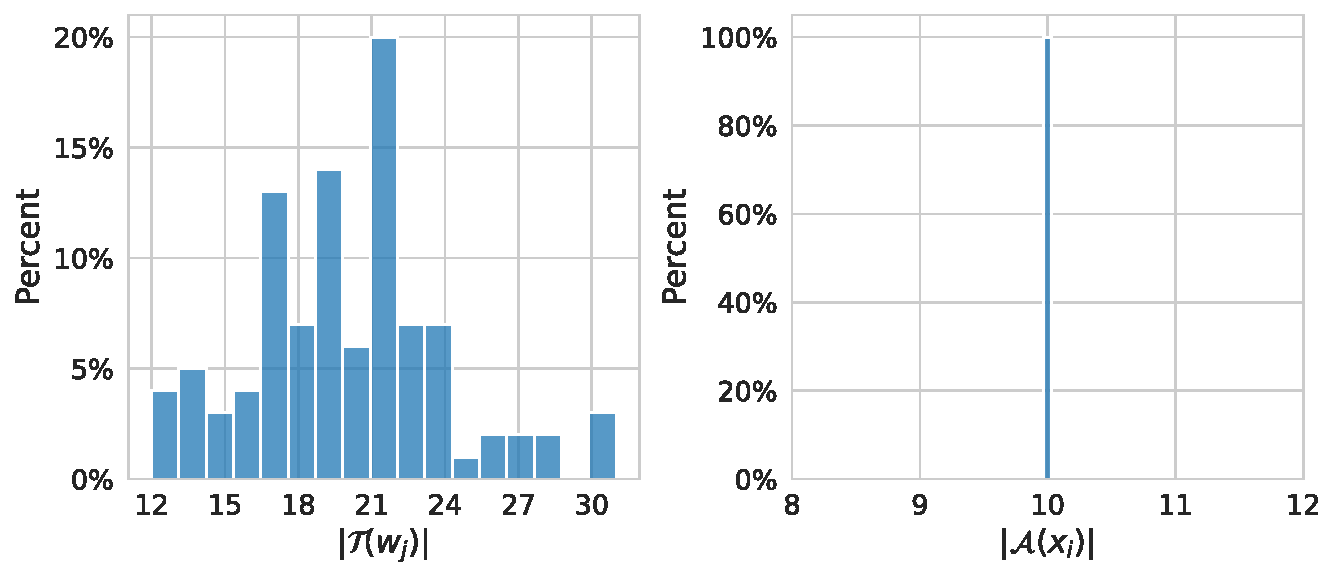
\includegraphics[width=.8\textwidth]{./chapters/images_peerannot/cell-20-output-1.pdf}
    \caption{Distribution of the number of tasks given per worker (left) and of the number of labels per task (right) in the setting with simulated discrete difficulty levels.}
\end{figure}

\begin{listing}[ht]
    \begin{minted}[linenos=true, bgcolor=lightgray, tabsize=4, fontfamily=courier, fontsize=\small, xleftmargin=5pt, xrightmargin=5pt]{python}
class Dawid_Skene(CrowdModel):
    def __init__(self, answers, n_classes, **kwargs):
        super().__init__(answers)
        ...

    def get_crowd_matrix(self):
        ... # Convert json answers to tensor (task, worker, label)

    def init_T(self):
        ... # Initialize the confusion matrices

    def m_step(self):
        """Maximizing log likelihood
        Returns:
            p: (p_j)_j class marginals
            pi: confusion matrices
        """
        ...

    def e_step(self):
        """Estimate indicator variables
        Returns:
            T: New estimate for the labels (n_task, n_worker)
        """
        ...

    def log_likelihood(self):
        ... # Compute the log likelihood of the model

    def run(self, epsilon=1e-6, maxiter=50):
        self.get_crowd_matrix()
        self.init_T()
        k, eps, ll = 0, np.inf, []
        while k < maxiter and eps > epsilon:
            self.m_step()
            self.e_step()
            likeli = self.log_likelihood()
            ll.append(likeli)
            if len(ll) >= 2:
                eps = np.abs(ll[-1] - ll[-2])
            k += 1

    def get_probas(self):
        return self.T

    def get_answers(self):
        return np.vectorize(self.converter.inv_labels.get)(
            np.argmax(self.get_probas(), axis=1)
        )
\end{minted}
\caption{MWE for the DS label aggregation in \texttt{peerannot}.}
\label{listing:DS}
\end{listing}

\chapter{Résumé et partie de l'introduction en français}
\label{chap:vf}

\section{Résumé}
Alors que les ensembles de données de classification sont composés d'un nombre croissant d'éléments, le besoin d'expertise humaine pour les étiqueter est toujours présent. Les plateformes d'apprentissage participatif sont un moyen de recueillir les commentaires d'experts à faible coût. Cependant, la qualité de ces étiquettes n'est pas toujours garantie. Dans cette thèse, nous nous concentrons sur le problème de l'ambiguïté des étiquettes dans l'apprentissage participatif. L'ambiguïté des étiquettes a principalement deux sources : la capacité du travailleur et la difficulté de la tâche. Nous présentons tout d'abord un nouvel indicateur, le $\mathrm{WAUM}$ (aire sous la marge pondérée), pour détecter les tâches ambiguës confiées aux travailleurs. Basé sur le $\mathrm{AUM}$ existant dans le cadre supervisé classique, il nous permet d'explorer de grands ensembles de données tout en nous concentrant sur les tâches qui pourraient nécessiter une expertise plus pertinente ou qui devraient être éliminées de l'ensemble de données actuel. Nous présentons ensuite une nouvelle bibliothèque \texttt{python} open-source, PeerAnnot, que nous avons développée pour traiter les ensembles de données en apprentissage participatif dans la classification d'images. Nous avons créé une référence d'état de performance dans la bibliothèque Benchopt pour évaluer nos stratégies d'agrégation d'étiquettes afin d'obtenir des résultats plus reproductibles. Enfin, nous présentons une étude de cas sur l'ensemble de données Pl@ntNet, où nous évaluons l'état actuel de la stratégie d'agrégation d'étiquettes de la plateforme et proposons des moyens de l'améliorer. Ce contexte avec un grand nombre de tâches, d'experts et de classes est très difficile pour les stratégies d'agrégation d'apprentissage participatif actuelles. Nous faisons état de performances systématiquement supérieures à celles de nos concurrents et proposons une nouvelle stratégie d'agrégation qui pourrait être utilisée à l'avenir pour améliorer la qualité de l'ensemble de données Pl@ntNet. Nous publions également ce grand ensemble de données de commentaires d'experts qui pourrait être utilisé pour améliorer la qualité des méthodes d'agrégation actuelles et fournir un nouveau point de référence.

\section{Introduction: apprentissage participatif en classification d'images}

Suite à la révolution de l'apprentissage profond, on entraîne aujourd'hui des modèles avec des millions voire des milliards de paramètres à optimiser. Et pour ce faire, nous avons besoin d'augmenter la taille de nos ensembles de données d'entraînement.
Le problème est que dans un ensemble d'entraînement en classification supervisée (et nous considérerons principalement la classification d'images pour le reste de ce travail), les images doivent être accompagnées d'une étiquette à partir de laquelle l'entraînement est effectué.
Bien que des recherches aient été menéees sur l'inférence de cette étiquette à partir des données elles-mêmes, dans les ensembles de données classiques d'apprentissage supervisé, ces étiquettes ont été collectées et partagées à un moment donné au cours de la création de l'ensemble de données.

\begin{figure}[ht]
    \centering
    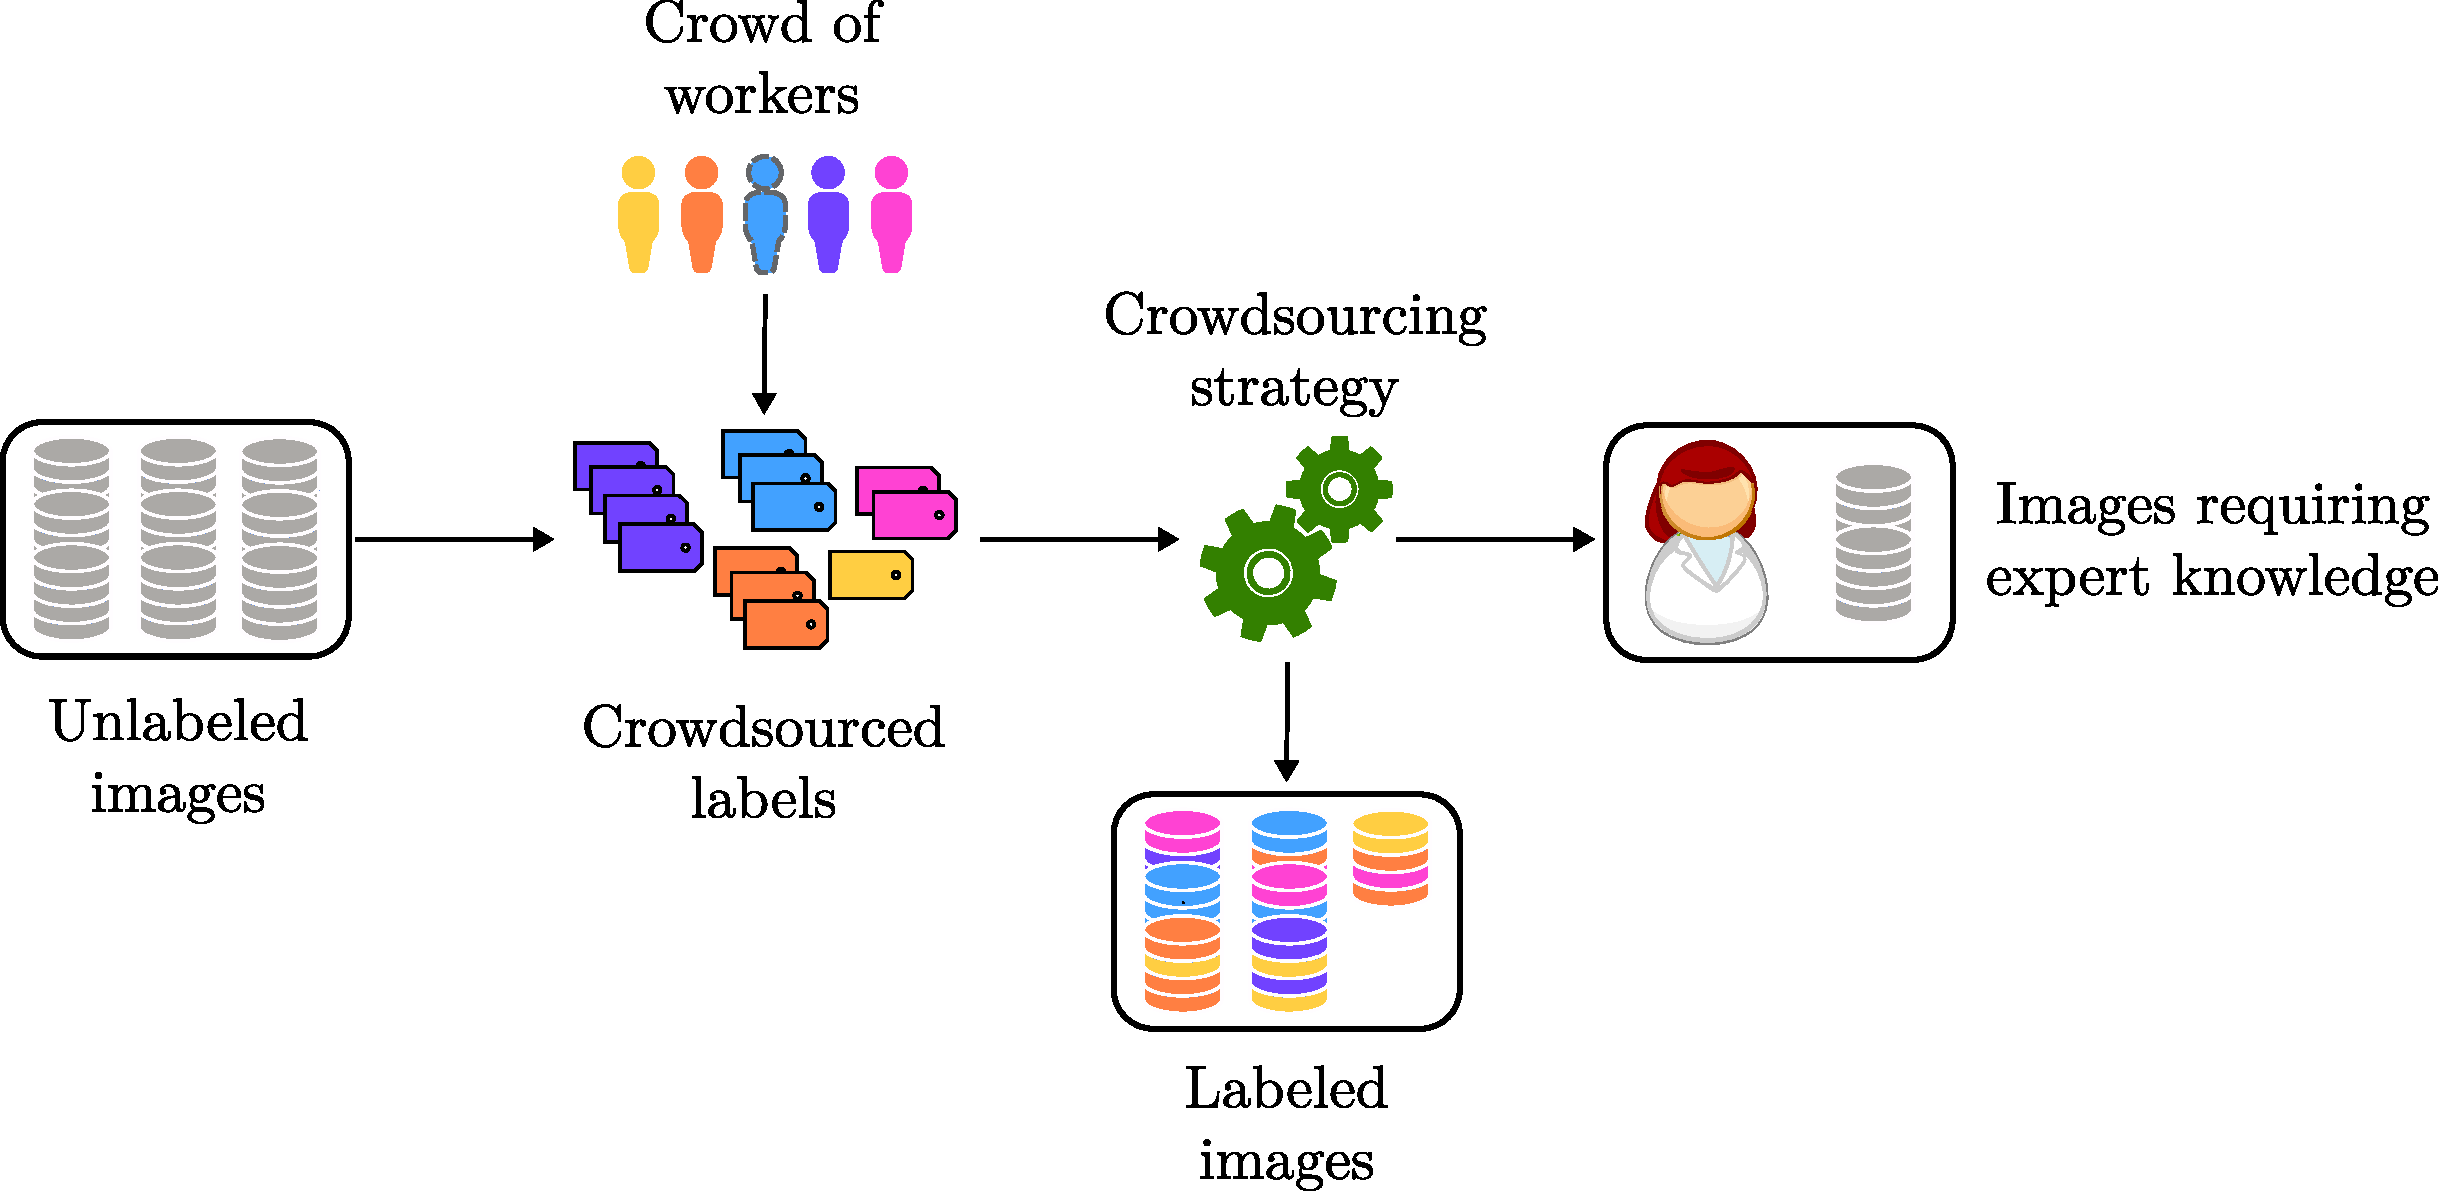
\includegraphics[width=.8\textwidth]{chapters/images/expert_knowledge.pdf}
    \caption{L'apprentissage participatif peut être utilisé pour créer des ensembles de données, mais il permet également de soulager la tension que subissent les experts lorsqu'ils évaluent de nouvelles données. En faisant appel à une foule de travailleurs, de nombreuses tâches peuvent être étiquetées sans nécessiter l'évaluation d'un expert.}
\end{figure}

La tâche consistant à collecter des données afin de créer un ensemble de données pour la classification des images a été de plus en plus associée à l'extraction automatique de données en ligne \citep{rhodes2015vaping}.
Toutefois, il a été démontré à de nombreuses reprises que cette stratégie de collecte de données entraîne des erreurs d'étiquetage \citep{northcutt_pervasive_2021,vasudevan2022does}.
Dans d'autres domaines de recherche, comme les prestataires de soins de santé, les images ne proviennent pas nécessairement du web mais sont collectées à plusieurs endroits, comme les scanners des hôpitaux.
Lorsqu'il s'agit de classer un scanner comme "présence ou absence de tumeurs", c'est souvent un expert sur le terrain qui fournit l'étiquette.
Cependant, ces professionnels de la santé ne peuvent pas étiqueter des milliers d'images.
Dans ce cas, la puissance de la foule peut être utilisée pour étiqueter les scanners et fournir un certain niveau d'incertitude.
Il appartient alors au scientifique des données, en collaboration avec les experts, de déterminer quels travailleurs ont été utiles dans l'expérience et lesquels ne l'ont pas été, puis de demander aux experts d'étiqueter uniquement les scans les plus ambigus - qui ne représenteraient qu'une petite fraction de l'ensemble de données original (comme illustré dans \Cref{fig:expert_knowledge}).

\subsection{Le crowdsourcing est partout}

Cette collaboration entre citoyens et scientifiques n'est pas une niche technique, mais elle passe souvent inaperçue.
L'utilisation du crowdsourcing pour collecter des données a été utilisée en médecine, dans les systèmes de recommandation vidéo, et dans bien d'autres domaines de la recherche et du développement.
Nous souhaitons présenter une liste - non exhaustive et non ordonnée - de ces projets qui s'appuient sur les interactions humaines pour collecter des données, et pas seulement pour la classification d'images :
\begin{itemize}
    \item Pl@ntNet : application de reconnaissance des espèces végétales \citep{plantet},
    \item Eyewire : un jeu pour cartographier les neurones de la rétine \citep{tinati2017investigation},
    \item Tournesol : système de recommandation de vidéos d'intérêt public sur YouTube \citep{hoang2021tournesol},
    \citep{openai2023gpt4}, \citep{openai2023gpt4}, \citep{openai2023gpt4}, \citep{openai2023gpt4},
    \item Duolingo : corrections de traduction et améliorations\footnote{\url{https://www.theguardian.com/education/2014/aug/27/luis-von-ahn-ceo-duolingo-interview}},
    \item RTR : segmentation des panneaux photovoltaïques dans les images \citep{kasmi2023crowdsourced},
    \item Twitter/$\mathbb{X}$ via Birdwatch : identifier les informations trompeuses \citep{wojcik2022birdwatch},
    \item Spotify\footnote{\url{https://community.spotify.com/t5/Content-Questions/Shutting-down-Line-In/td-p/4557664}}, TripAdvisor\footnote{\url{https://www.kingigilbert.com/crowdsourcing-tripadvisor/}}, SNCF\footnote{\url{https://www.usine-digitale.fr/article/tranquilien-quand-open-data-et-crowdsourcing-profitent-aux-voyageurs-franciliens.N200017}},\dots
\end{itemize}

Avec cette liste, nous mettons en évidence les vastes domaines d'application qui permettent aux humains - et aux citoyens - de rester dans la boucle, et donc la nécessité de poursuivre les recherches sur les paramètres, les stratégies et les implications du crowdsourcing.
Dans cette thèse, nous nous concentrons principalement sur la classification d'images.

\subsection{Le projet de Pl@ntNet}
Créé par Alexis Joly et Pierre Bonnet, Pl@ntNet \citep{plantet} est la rencontre de deux communautés -- les botanistes et l'informatique -- pour identifier des espèces végétales à partir de photos prises sur le vif.
Le projet est né en 2008, a sorti sa première application web en 2011, son application mobile en 2013 et a reçu en 2020 le prix \emph{Prix de l'innovation Inria - Académie des sciences - Dassault Systèmes}.
\begin{figure}[tbh]
    \centering
    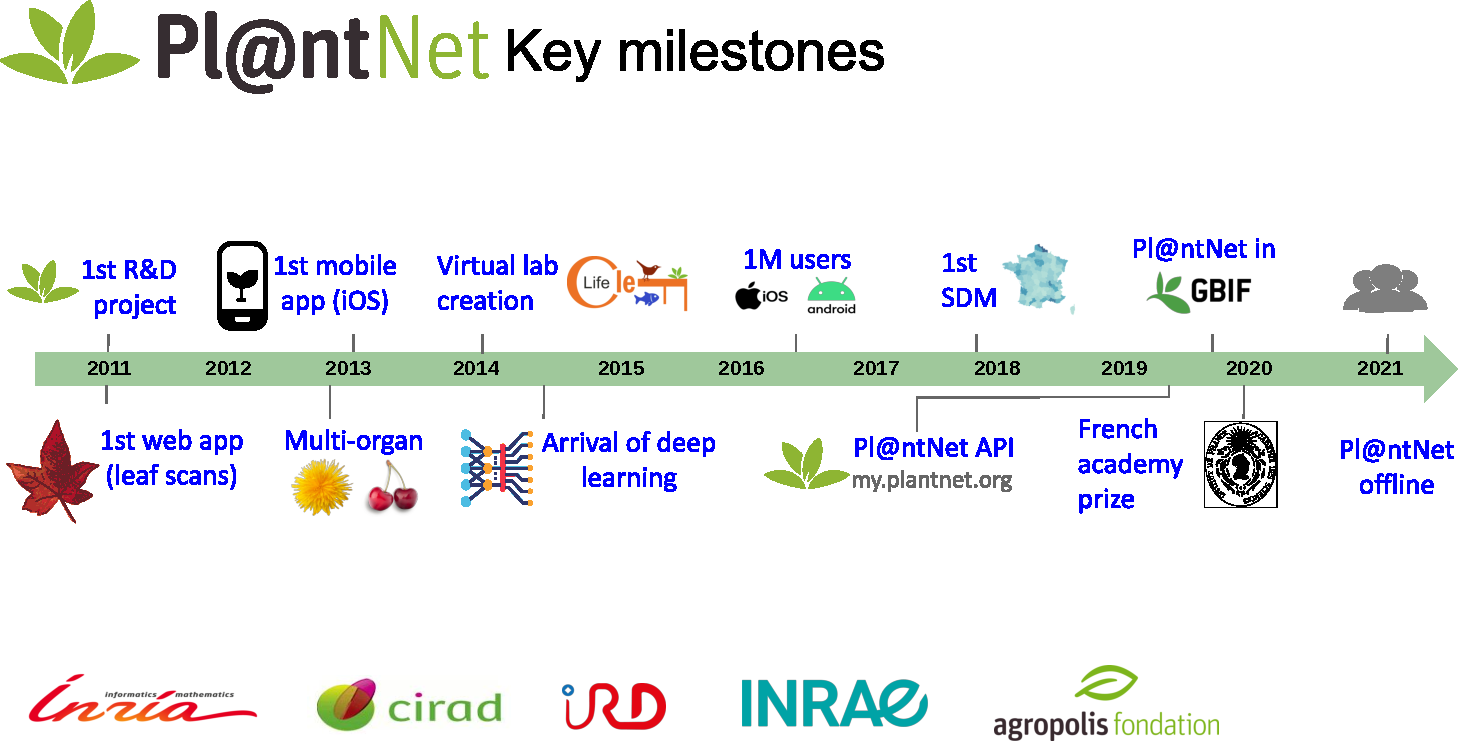
\includegraphics[width=.8\textwidth, clip, trim={0cm 0cm 0cm 2.5cm}]{chapters/images/Pl@ntNet-overview-Janv-2022.pdf}
    \caption{Timeline du projet Pl@ntNet}
    \label{fig:timeline-plantnet}
\end{figure}

Le système Pl@ntNet peut être interprété comme suit. Un utilisateur enregistre une observation (une image ou un groupe d'images de la même plante) et envoie une requête d'identification.
La version actuelle du modèle de vision par ordinateur de Pl@ntNet (appelé modèle IA de Pl@ntNet et détaillé dans \Cref{chap:plantnet}) fait une prédiction et fournit l'espèce la plus probable.
L'utilisateur peut alors approuver le modèle d'IA ou saisir une autre espèce.
Avec les probabilités prédites, des observations similaires avec les espèces indiquées sont montrées à l'utilisateur pour l'aider à prendre sa décision.
L'observation est ensuite partagée (avec l'accord de l'utilisateur) avec la communauté et peut faire l'objet d'un vote de la part des autres utilisateurs/

\begin{figure}[htb]
    \centering
    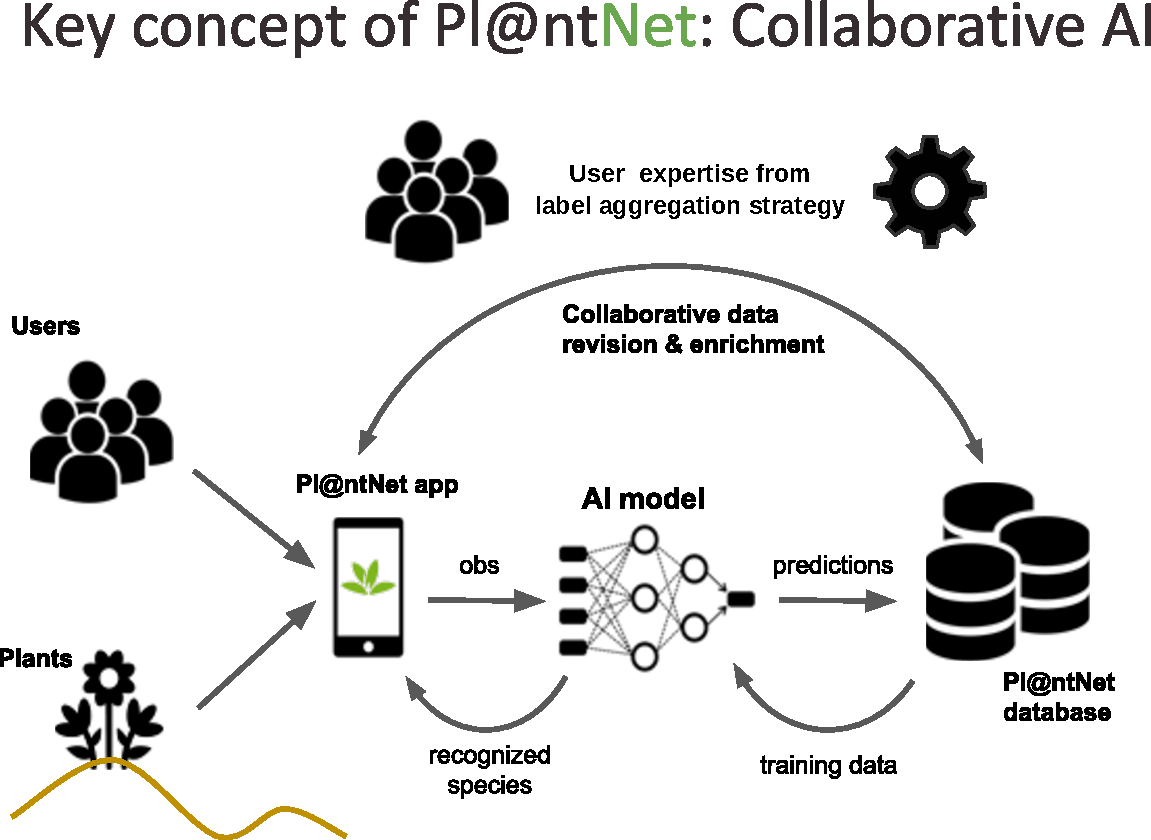
\includegraphics[width=.65\textwidth, clip, trim={0cm 0cm 0cm 2cm}]{chapters/images/cooperative learning Pl@ntNet schema.pdf}
    \caption{Pl@ntNet pipeline from the observation taken in the field to the active training of the computer vision model.}
\end{figure}

Une fois l'observation enregistrée, elle peut être révisée à tout moment par d'autres utilisateurs.
Actuellement, Pl@ntNet enregistre plus de $50$K espèces, $6$M utilisateurs enregistrés et $21$M observations réparties sur $77$ flores.
Plus d'un milliard de requêtes d'images ont été effectuées et l'application a été téléchargée plus de 10 millions de fois sur Google AppStore.
Au total, plus de 22 millions de votes ont été exprimés au niveau international.
Chaque observation partagée publiquement présente, comme dans \Cref{fig:interface-plantnet} avec un auteur associé, les votes actuels et l'état de la détermination actuelle de l'espèce.
Sur la plateforme, les utilisateurs peuvent voter pour une étiquette malformée, si l'image concerne une feuille, une fleur, un fruit, l'écorce, le port ou autre. Dans cette thèse, nous ne prenons en compte que la détermination de l'espèce, et non les autres votes.

\begin{figure}[H]
    \centering
    \begin{minipage}{.55\linewidth}
        \centering
        \subfloat[Identification webpage. L'observation est composée de deux images, l'une de l'organe (à gauche) et l'autre de la fleur (à droite).]{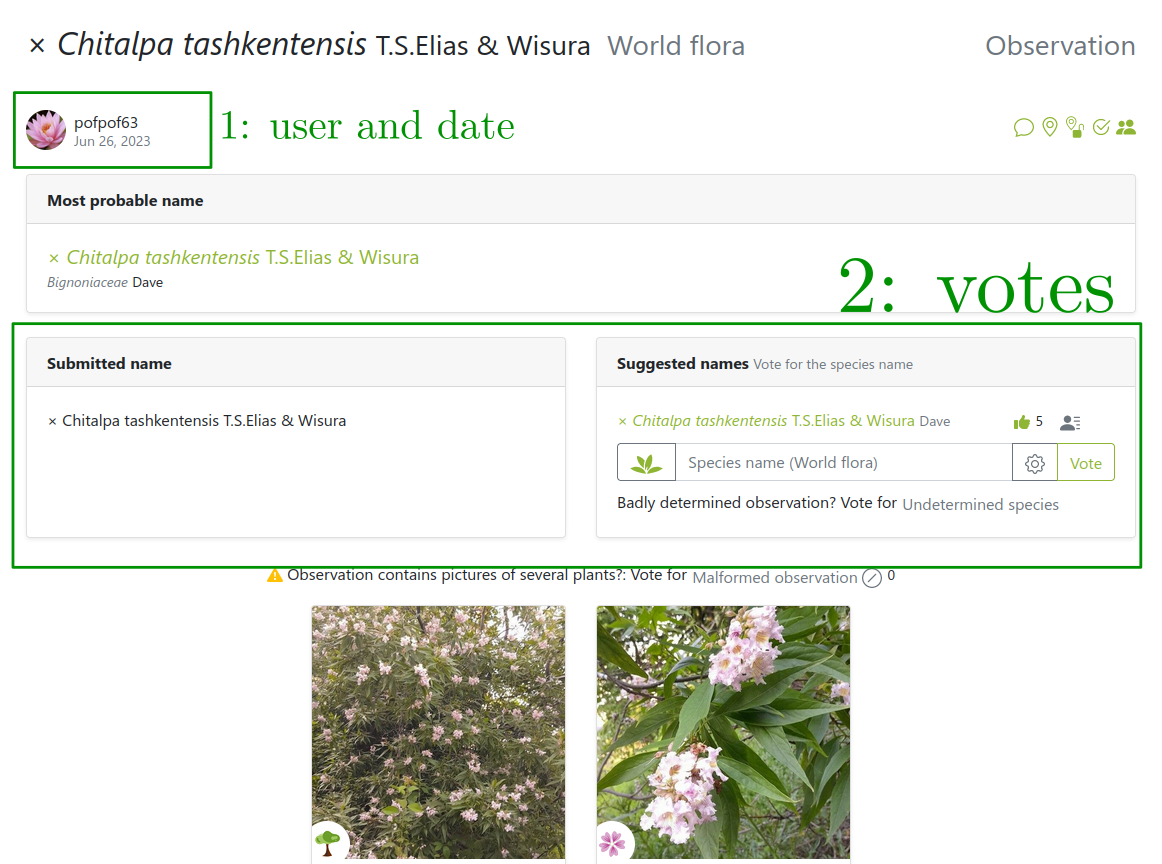
\includegraphics[width=\textwidth]{chapters/images/plantnet_online.png}}
    \end{minipage}%
        \hfill
    \begin{minipage}{.4\linewidth}
        \centering
        \subfloat[Vision de l'utilisateur sur les prédictions du modèle actuel. Des exemples pour chaque espèce sont proposés à des fins de comparaison visuelle.]{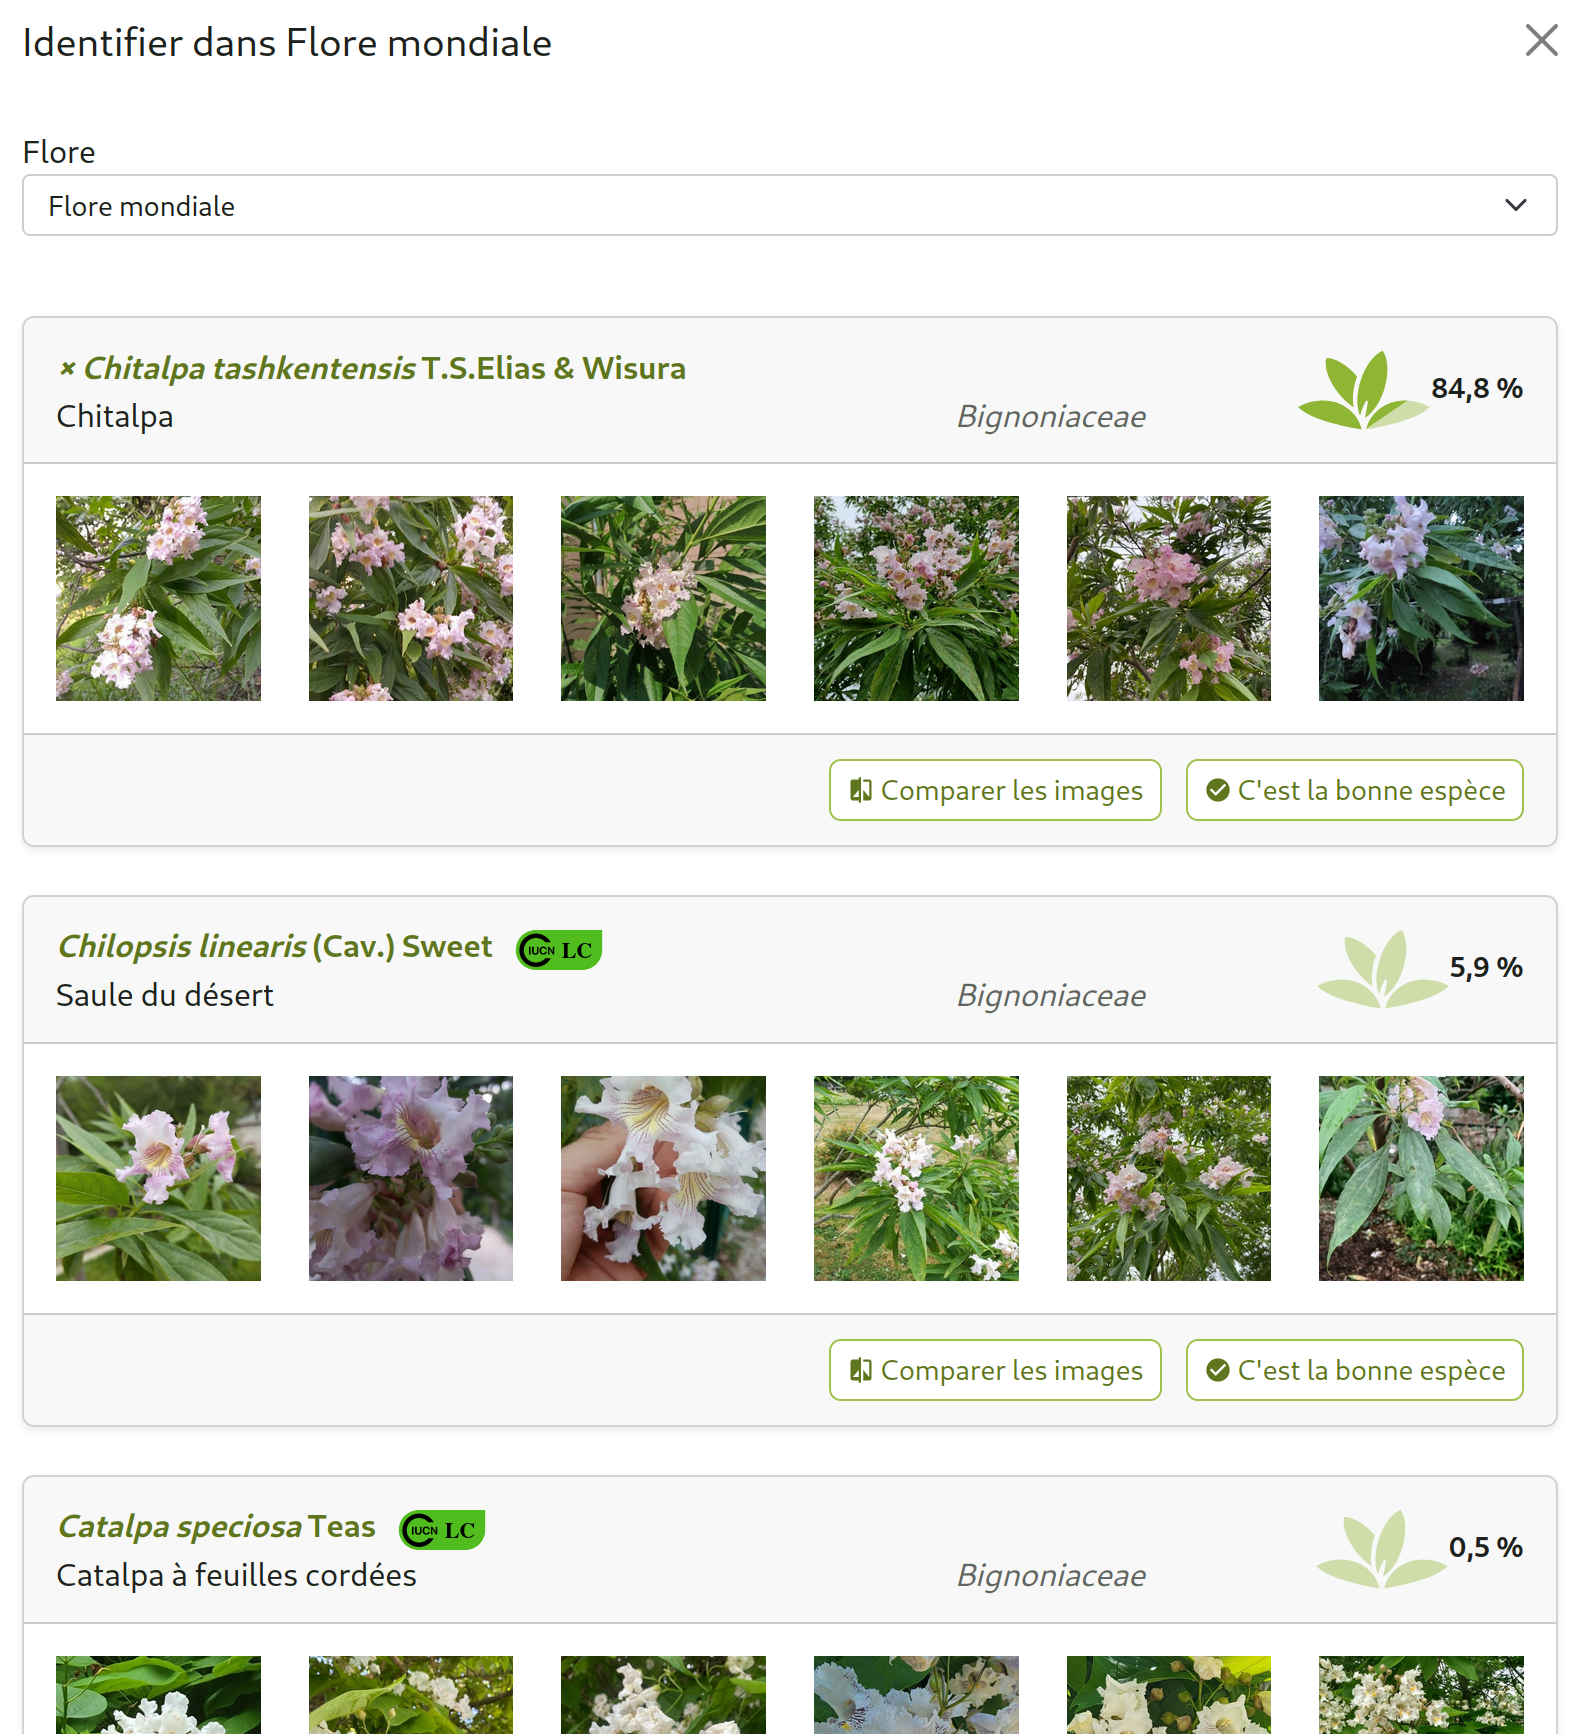
\includegraphics[width=\textwidth]{chapters/images/AI_votes.png}}
    \end{minipage}\par\medskip
        \caption{Exemple d'observation à partir de l'interface en ligne de Pl@ntNet. L'utilisateur représenté est l'auteur de l'observation. Nous enregistrons le nom de l'espèce initialement soumis, ainsi que les différents votes (ici, 5 utilisateurs sont d'accord sur la détermination de l'étiquette). Si les images d'une observation ne contiennent pas la même plante, les utilisateurs peuvent voter pour une étiquette malformée. En cliquant sur l'icône près du champ d'identification, les utilisateurs peuvent voir la prédiction actuelle du modèle de vision par ordinateur.}
    \end{figure}


Lors du vote, les utilisateurs voient apparaître la prédiction actuelle de vision par ordinateur sur l'observation -- comme indiqué dans \Cref{fig:interface-ai}. Cette prédiction influence le vote des utilisateurs, mais contient également des informations.
Au moment de la rédaction de ce document, le modèle de vision par ordinateur de Pl@ntNet est un réseau DINOv2 \citep{oquab2024dinov2} basé sur des transformateurs.
En utilisant l'apprentissage contrastif \citep{waida2023understanding} \emph{i.e.} représentant des images similaires sous forme d'encastrement proche pour apprendre des caractéristiques similaires pour des observations similaires, puis en utilisant l'apprentissage supervisé pour affiner le modèle.

Dans \Cref{chap:plantnet}, nous présentons la stratégie d'agrégation des étiquettes de Pl@ntNet, mais aussi la manière dont nous pouvons incorporer les prédictions du modèle dans l'agrégation des étiquettes.
La prise en compte du vote du réseau est une question délicate, car nous ne voulons pas que l'IA devienne trop confiante dans ses prédictions en s'appuyant principalement sur ses prédictions et en écartant les votes humains.
L'expertise humaine étant l'objectif principal de la plateforme, nous voulons garder les humains dans la boucle, en particulier les experts botaniques, afin de continuer à améliorer les identifications de plantes des utilisateurs finaux.

